\newpage

\section{Reti Bayesiane}

Sono dei modelli utili in situazioni di \textbf{incertezza}.\\

\textbf{Esempio}

Si modella la seguente situazione\dots

\begin{itemize}
\item L'allarme di casa (\textbf{A}) può scattare a causa di un terremoto
(\textbf{E})
\item L'allarme di casa (\textbf{A}) può scattare a causa di un'intrusione
(\textbf{B})
\item L'allarme di casa (\textbf{A}) acceso può portare Mary (\textbf{M}) o
John (\textbf{J}) a chiamarmi
\end{itemize}

Le variabili del problema sono state riportate fra parentesi in grassetto:
A, E, B, M, J.
La rete bayesiana che rappresenta la situazione è rappresentata in figura
\ref{fig:alarm}:

\begin{figure}[H]
\centering
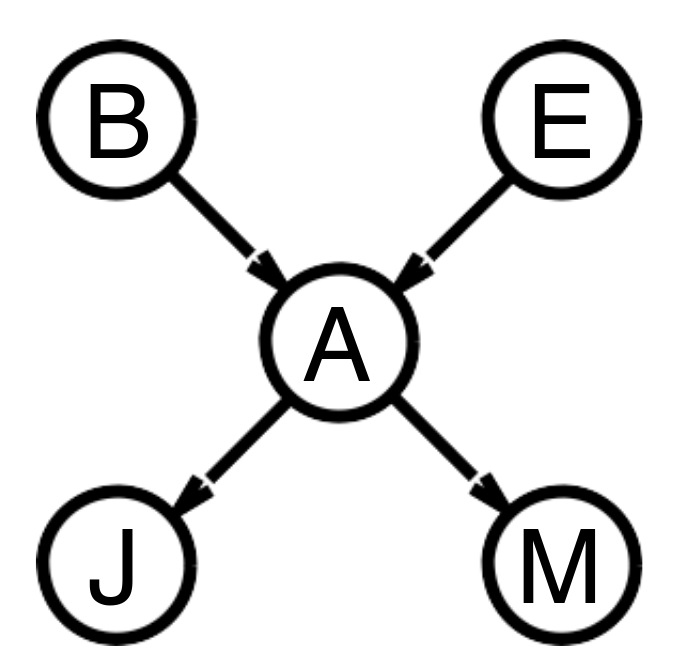
\includegraphics[width=0.22\textwidth]{alarm}
\caption{Rete bayesiana che modella l'esempio precedente}
\label{fig:alarm}
\end{figure}

\subsection{Sintassi delle reti bayesiane}

Gli archi rappresentano le \textbf{dipendenze} tra le variabili (nodi):
$X \rightarrow Y$ significa che X influenza direttamente Y.

Una rete bayesiana è un \textbf{grafo orientato senza cicli}.

Ciascun nodo/variabile/evento ha una certa probabilità di verificarsi,
data la probabilità dei suoi genitori.

Questa viene detta probabilità condizionata ed è rappresentata tramite
delle tabelle di distribuzione di probabilità condizionata \textbf{CPT}.
Nell'immagine \ref{fig:cpt} le CPT vengono associate ai nodi della rete
bayesiana dell'esempio:

\begin{figure}[H]
\centering
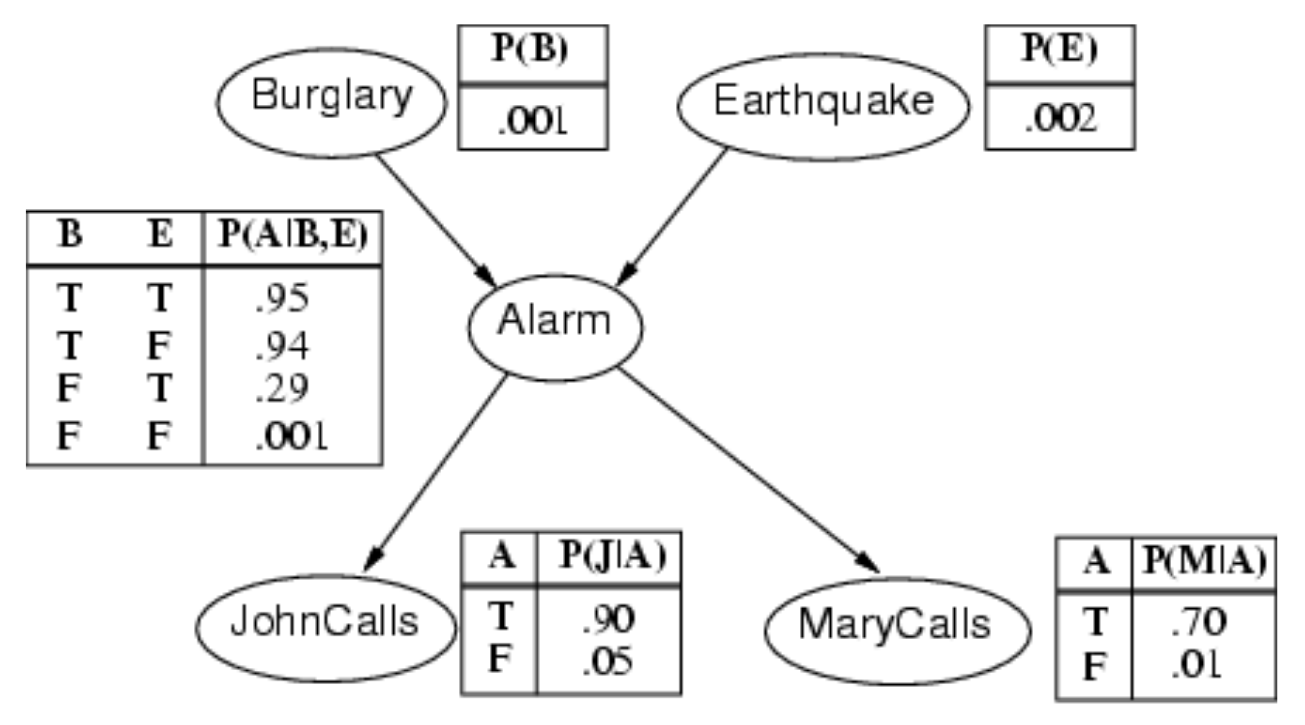
\includegraphics[width=0.65\textwidth]{cpt}
\caption{Rete bayesiana con CPTs}
\label{fig:cpt}
\end{figure}

\textbf{Nota}: le probabilità iniziali P(B) e P(E) sono le probabilità
che B ed E si verifichino (siano veri). Per trovare le probabilità che
B ed E siano falsi basta semplicemente fare il calcolo 1 - P(B) o 1 -
P(E).\\

Una CPT per una variabile booleana $X_i$ con k genitori ha $2^k$ righe
(date le combinazioni dei genitori). Con n variabili/nodi sono quindi
richieste $n2^k$ righe

Nella rete bayesiana dell'esempio quante righe ci sono? Basta fare il
conto: $1 (E) + 1 (B) + 2^2 (A) + 2^1 (J) + 2^1 (M) = 1 + 1 + 4 + 2 + 2
= 10$ righe.

\subsection{Semantica delle reti bayesiane}

Nella \textbf{full joint distribution} occorre tenere conto di tutte
le combinazioni possibili. Nell'esempio ci sono 5 variabili, quindi
$2^5 = 32$ numeri.

La full joint distribution viene definita come il prodotto delle
distribuzioni di probabilità condizionata locali: 

\begin{equation}
 P(x_1, ..., x_n) = \prod_{i=1}^n P(X_i | Parents(X_i))
\end{equation}

Applicando la formula precedente, ad esempio, si può calcolare
la probabilità che l'allarme sia scattato e che sia John che Mary
abbiano chiamato, ma non si siano verificati né un terremoto né un'
intrusione:\\

Convenzione: $P(X = true) = P(x)$

$P(j \land m \land a \land \neg b \land \neg e) = P(j|a)P(m|a)
P(a|\neg b, \neg e) P(\neg b) P(\neg e)$.\\

Svolgendo tutti i calcoli risulta che questa probabilità sia 0.000628
(molto bassa).

\subsection{Come costruire una rete Bayesiana?}

\begin{itemize}
 \item Scegliere un ordinamento delle variabili
 \item \texttt{for i = 1 to n do}\dots
 \item aggiungi $X_i$ alla rete e\dots
 \item scegli i suoi genitori in modo tale che
 $P(X_i | Parents(X_i)) = P(X_i| X_1, ..., X_{i-1})$
\end{itemize}

\subsection{Inferenza}

L'inferenza probabilistica permette di conoscere la distribuzione di
probabilità di un certo insieme di eventi di output, dato un insieme di
eventi in input.\\

Gli eventi di input vengono chiamati \textit{evidence variables}, mentre
gli eventi di output vengono chiamati \textit{query variables}. Tutti gli
eventi che non sono né input né output sono \textit{hidden variables}.

L'output dell'inferenza probabilistica è una full-joint distribution
sulle query variables:

$P(Q_1,..., Q_n| E_1 = e_1,..., E_n = e_n)$\\

Esistono 2 modi per fare inferenza probabilistica in una rete bayesiana:
attraverso un'enumerazione o eliminazione di variabili.\\

\subsubsection{Inferenza per enumerazione}

\textbf{Esempio di enumerazione}: si vuole trovare la probabilità che ci
sia stata un'intrusione, sapendo che sia John che Mary hanno chiamato.

In questo esempio, b è la query variables mentre j e m sono le evidence
variables.

Dalla definizione di probabilità condizionata segue che:

\begin{equation}
\label{eq:pc}
P(E_2|E_1) = \frac{P(E_1, E_2)}{P(E_1)}
\end{equation}

$P(b|j,m)$ (applicando l'equazione \ref{eq:pc}) $= \frac{P(b,j,m)}{P(j,m)} =
\alpha P(b,j,m)$, dove $\alpha = \frac{1}{P(j,m)}$

La probabilità $P(b,j,m)$ può essere determinata enumerando tutti possibili
valori delle hidden variables a,e:

$P(b,j,m) = \sum_e \sum_a P(b,j,m)$ (riscrivendo l'espressione considerando
la rete bayesiana e i genitori delle variabili) $= \sum_e \sum_a P(b)P(e)
P(a|b,e)P(j|a)P(m|a) = \alpha P(b) \sum_e P(e) \sum_a P(a|b,e)P(j|a)P(m|a)$

Quest'espressione va calcolata considerando tutte le possibilità delle
hidden variables che si stanno sommando (cioè $e, \neg e, a, \neg a$).

L'albero di valutazione completo dell'espressione è rappresentato in figura
\ref{fig:evalIS}. La complessità dell'inferenza per enumerazione è di
$\mathcal{O}(n2^n)$. Questo metodo NON è efficiente in quanto si ripetono i
rami per j e m

\begin{figure}[H]
\centering
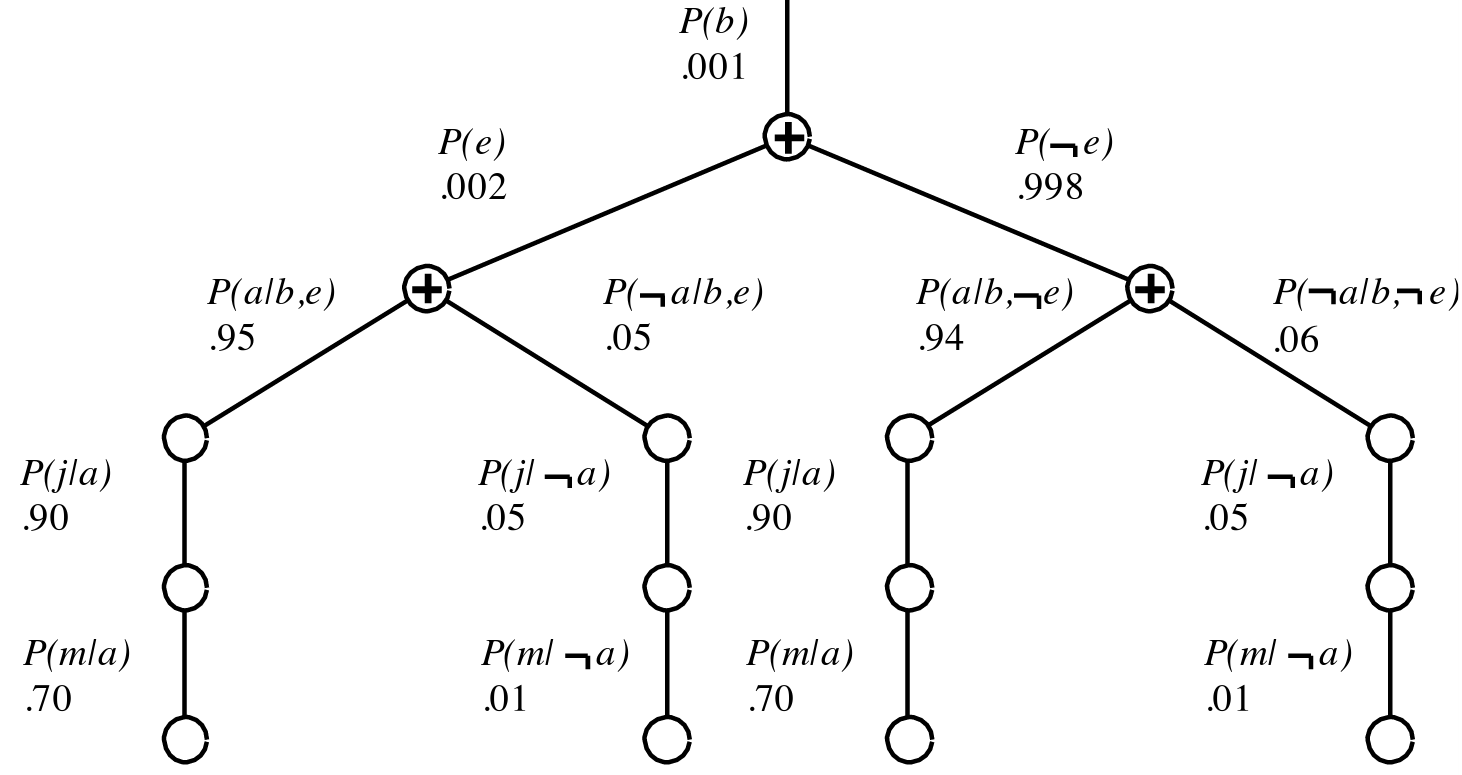
\includegraphics[width=0.8\textwidth]{evalIS}
\caption{La valutazione dell'espressione che calcola P(b,j,m). Si procede
top-down, moltiplicando i valori lungo un cammino e sommando ai nodi +.
Questo metodo NON è efficiente in quanto si ripetono i rami per j e m.}
\label{fig:evalIS}
\end{figure}

\subsubsection{Inferenza per eliminazione di variabili}

Come si può notare dalla figura \ref{fig:evalIS} l'inferenza per
enumerazione può essere migliorata evitando di ripetere calcoli.

L'algoritmo di eliminazione di variabili valuta espressioni come:\\

$P(b,j,m) = \alpha P(b) \sum_e P(e) \sum_a P(a|b,e)P(j|a)P(m|a)$
\textbf{da destra a sinistra}.\\

L'espressione può essere vista come un prodotto dei seguenti fattori:\\

$P(b|j,m) = \alpha f_1(B)$ x $\sum_e f_2(E)$ x $\sum_a f_3(A,B,E)$ x $f_4(A)
x f_5(A)$\\

L'operatore x utilizzato è il \textbf{pointwise product}.

Siano X e Y due insiemi e sia la moltiplicazione un operatore ben
definito in Y, cioè: $. : Y$ x $Y \rightarrow Y$ che rispetta la
definizione di funzione.

Siano f e g due funzioni f,g: $X \rightarrow Y$. Allora il prodotto
pointwise $(f\cdot g): X \rightarrow Y$ è così definito:

$(f\cdot g)(x) = f(x)\cdot g(x)$ per ogni x in X.\\
 
Ogni fattore è una matrice indicizzata dalla/e variabile/i condizionate a
cui si riferisce e che possono essere reperite dalla rete bayesiana.\\

La valutazione dell'espressione avviene da destra a sinistra: dapprima 
si calcola $f_6(B,E) = \sum_a f_3(a,b,e)$ x $f_4(a)$ x $f_5(a) = (f_3(a,b,e)$ x
$f_4(a) x f_5(a))$ + $(f_3(\neg a,b,e)$ x $f_4(\neg a)$ x $f_5(\neg a))$\\

poi si calcola\dots\\

$f_7(B) = \sum_e f_2(E)$ x $f_6(B,E) = (f_2(e)$ x $f_6(b,e)) + (f_2(\neg e)$ x
$f_6(b, \neg e))$.\\

L'espressione risultante è la seguente: $P(B|j,m) = \alpha f_1(B)$ x $f_7(B)$.

La somma delle matrici è quella usuale, un piccolo accorgimento è quello di
ricordarsi di portare fuori dalla somma i fattori che non dipendono dalle
variabili sommate.

\subsection{Esercizio}

Consider the BN shown in the figure below. Compute the probability
P(D|+b) \textbf{by enumeration} (you don't need to compute the normalization
factor $\alpha$).

Notazione: $P(E = true) = P(+e)$

\begin{figure}[H]
\centering
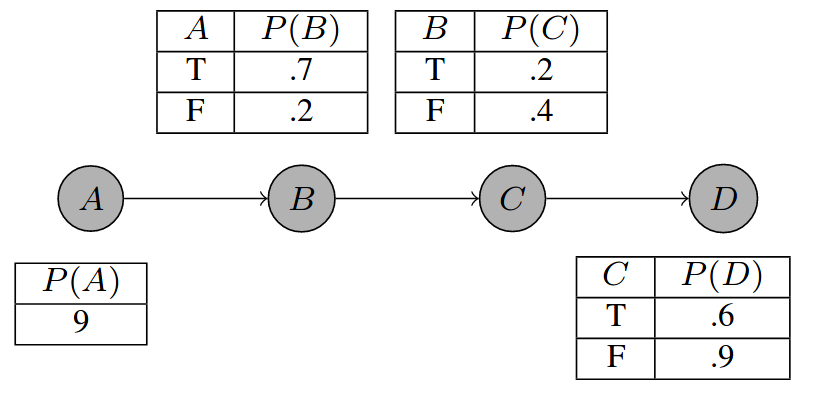
\includegraphics[width=0.65\textwidth]{bayesEx}
\caption{Rete bayesiana dell'esercizio}
\label{fig:bayesEx}
\end{figure}

$P(D|+b)$ è una distribuzione di probabilità e si ottiene calcolando $P(+d|+b)$ e
$P(\neg d|+b)$.\\

Calcolo di $P(+d|+b)$ tramite enumerazione:\\

$P(+d|+b) \propto P(+d, +b) = \sum_a P(a) P(+b|a) \sum_c P(c|+b) P(+d|c) =
[P(+a)P(+b|+a) + P(\neg a) P(+b|\neg a)][P(+c|+b) P(+d|+c) + P(\neg c|+b)
P(+d|\neg c)] = (0.9\cdot 0.7 + 0.1\cdot 0.2)\cdot (0.2\cdot 0.6 + 0.8\cdot 0.9) =
0.546$\\

Calcolo di $P(D|+b)$ tramite eliminazione:\\

$P(D|+b) \propto P(D, +b) = \sum_a P(a) P(+b|a) \sum_c P(c|+b) P(D|c) =
\sum_a f_1 (a)$ x $f_2 (a)$ x $\sum_c f_3 (c)$ x $f_4 (D, c)$\\

Calcolo $f_5 (D) = \sum_c f_3 (c)$ x $f_4 (D, c) = f_3 (+c)$ x $f_4 (D, +c)$ +
$f_3 (\neg c)$ x $f_4 (D, \neg c)$\\

$f_3 (+c) = 0.2$

$f_4 (D, +c) =
\begin{bmatrix}
0.6 \\
0.4
\end{bmatrix}$

$f_3 (\neg c) = 0.8$

$f_4 (D, \neg c) =
\begin{bmatrix}
0.9 \\
0.1
\end{bmatrix}$\\

$f_5 (D) =
\begin{bmatrix}
0.12 \\
0.08
\end{bmatrix} + 
\begin{bmatrix}
0.72 \\
0.08
\end{bmatrix} =
\begin{bmatrix}
0.84 \\
0.16
\end{bmatrix}$
\\

Calcolo $f_6 = \sum_a f_1 (a)$ x $f_2 (a) = f_1 (+a)$ x $f_2 (+a)$ +
$f_1 (\neg a)$ x $f_2 (\neg a)$\\

$f_1 (+a) = 0.9$

$f_2 (+a) = 0.7$

$f_1 (\neg a) = 0.1$

$f_2 (\neg a) = 0.2$

$f_6 = 0.9\cdot 0.7 + 0.1\cdot 0.2 = 0.63 + 0.02 = 0.65$\\

Quindi $P(D, +b) = 
\begin{bmatrix}
0.84 \\
0.16
\end{bmatrix}
\cdot 0.65 =
\begin{bmatrix}
0.546 = P(+d, +b) \propto P(+d|+b) \\
0.104 = P(\neg d, +b) \propto P(\neg d|+b)
\end{bmatrix}$
